\documentclass[a4paper]{article}
\usepackage{amsmath}
\usepackage{amsthm}
\usepackage{amsfonts}
\usepackage{color}
\usepackage{graphicx}
\usepackage{listings}

\newcommand{\R}{\mathbb{R}}

%opening
\title{3D Incompressible Navier-Stokes using FreeFEM++}
\author{Afifah Maya Iknaningrum}

\begin{document}

\lstset{
	language=C,                % choose the language of the code
	numbers=left,                   % where to put the line-numbers
	stepnumber=1,                   % the step between two line-numbers.        
	numbersep=5pt,                  % how far the line-numbers are from the code
	backgroundcolor=\color{white},  % choose the background color. You must add \usepackage{color}
	showspaces=false,               % show spaces adding particular underscores
	showstringspaces=false,         % underline spaces within strings
	showtabs=false,                 % show tabs within strings adding particular underscores
	tabsize=2,                      % sets default tabsize to 2 spaces
	captionpos=b,                   % sets the caption-position to bottom
	breaklines=true,                % sets automatic line breaking
	breakatwhitespace=true,         % sets if automatic breaks should only happen at whitespace
	title=\lstname,                 % show the filename of files included with \lstinputlisting;
}

\maketitle

\begin{abstract}
-
\end{abstract}

\section{Introduction}

Navier-Stokes equation is considered as one of nonlinear equations that holds important rule in fluid mechanics. It can describe interesting phenomena of flow of viscous fluid like tornado. By understanding the behavior of tornadoes, we can study how to prevent greater loss when its happened.

In this research, using Finite Element Method (FEM) and software FreeFEM++, the 3D simulations of tornadoes is disscussed. First, considering cubes domain, better choice of time-step and time-discretization method is determined. Then changing the domain, the simulation is done in the cylindrical domain. Given initial condition with swirl and without swirl for tornado, simulation in cylindrical and curved cylindrical domain is disscussed.

\subsection{Problem}
Solving Navier-Stokes equations in FreeFEM++, the weak formulation of the equation is needed. In this research, the Incompressible condition term $ \nabla \cdot u = 0 $ is considered.
\subsubsection{Strong formulation}
We want to find \[(u,p) : \Omega \times (0,T) \rightarrow \R^3 \times \R\] where $ u $ is unknown velocity and $ p $ is unknown pressure with $ \nu > 0 $ is a viscosity, such that
\begin{equation}\label{Navier-Stokes}
\begin{cases}
\dfrac{\partial u}{\partial t} + (u \cdot \nabla) u - \nu \bigtriangleup u + \nabla p = f & \text{ in } \Omega \times (0,T)\\
\nabla \cdot u = 0 & \text{ in } \Omega \times (0,T)\\
u = 0 & \text{ on } \partial \Omega \times (0,T)\\
u = u^0 & \text{ in } \Omega \text{, at } t=0
\end{cases}
\end{equation}
where $ f : \Omega \times (0,T) \rightarrow \R^3 $ and $ u^0 : \Omega \rightarrow \R^3 $ are given functions.
\subsubsection{Weak formulation}
The weak formulation for equation (\ref{Navier-Stokes}) is shown below. We want to find $ \{ (u,p)(t) \in V \times Q ; t \in (0.T) \} $ such that for $ t \in (0,T) $
\begin{equation} \label{NS_Weak}
\begin{cases}
\big( \dfrac{\partial u}{\partial t} + (u \cdot \nabla)u,v \big) + a(u,v) + b(v,p) + b(u,q) = (f,v) & ,\forall(v,q)\in V\times Q \\ u=u^{0} & , t=0
\end{cases}
\end{equation}
where
\begin{eqnarray}\nonumber
a(u,v) &=& \nu \int_{\Omega} \nabla u : \nabla v \ dx \\ \nonumber
b(v,q) &=& - \int_{\Omega} (\nabla \cdot v) q \ dx \\ \nonumber
V &=& H_{0}^{1}(\Omega, \R^d) = H_{0}^{1}(\Omega)^d \\ \nonumber
Q &=& \{ q\in L^2(\Omega) ; \int_{\Omega} q \ dx=0 \}.
\end{eqnarray}

\subsection{Time discretization}
Before applying to FreeFEM++, we need to discritize $ \Big(\dfrac{\partial u_{i}}{\partial t} + (u \cdot \nabla)u_{i}\Big) $ part, with $ dt $ as time increment and convect field
\[ X_{1}(u_{i}^{n-1},dt)(x) = x - u_{i}^{n-1}(x)\ dt.\]
\subsubsection{First order}
Using backward scheme, 
\[ \dfrac{\partial u_{i}}{\partial t} + (u \cdot \nabla)u_{i} \approx \dfrac{u_{i}^{n}-u_{i}^{n-1}(X_{1}(u_{i}^{n-1},dt))}{dt} + O(dt) \]
\subsubsection{Second order}
Using Adam-Bashforth method,
\[\dfrac{\partial u_{i}}{\partial t} + (u \cdot \nabla)u_{i} \approx \dfrac{3u_{i}^{n}-4u_{i}^{n-1}(X_{1}(\tilde{u}_{i}^{n-1},dt))+u_{i}^{n-2}(X_{1}(\tilde{u}_{i}^{n-1},2dt))}{2\ dt} + O(dt^2)\]
with $ \tilde{u}_{i}^{n-1} = 2u_{i}^{n-1}-u_{i}^{n-2} $.
\subsection{Stabilization term}
With $ \delta>0 $ and $ h $ as mesh size, the stabilization term used is
\[ C_{i}(p,q) = \delta \sum_{k} h_{k}^{2}(\nabla p, \nabla q)_{k} \]

\subsection{Error estimate}
\subsubsection{$ L^{2} $ norm}
\[\| u_{h}^{n}-u^{n} \|_{\ell^\infty(L^2)} =  max \ \| u_{h}^{n}-u^{n} \|_{L^{2}}\]
with $ O(h^2) $.
\subsubsection{$ H^{1} $ norm}
\[\| u_{h}^{n}-u^{n} \|_{\ell^\infty(H^{1})} = max \sqrt{\| u_{h}^{n}-u^{n} \|_{L^2(\Omega)}^{2} + \| \nabla (u_{h}^{n}-u^{n}) \|_{L^2(\Omega)}^{2}}\]
with $ O(h) $.

\newpage
\section{Simulation with artificial solution}

\subsection{Cubic and cylindrical domain}
With the exact solution
\begin{eqnarray}\nonumber
u &=& (u_{1},u_{2},u_{3}) \\ \nonumber
u_{1} &=& -\cos(x_{1}) \sin(x_{2}) \cos(x_3) e^{-2t}\\ \nonumber
u_{2} &=& \sin(x_{1}) \cos(x_{2}) \cos(x_3) e^{-2t}\\ \nonumber
u_{3} &=& 0 \\ \nonumber
p&=& \dfrac{-1}{4} e^{-4t} (\cos(2x_1)+\cos(2x_2)+\cos(2x_3))
\end{eqnarray}
such that equation (\ref{Navier-Stokes}) is satisfied with $ f = (f_{1},f_{2},f_3) $
\begin{eqnarray}\nonumber
f_{1} &=& -\cos(x_1) \sin(x_2) \cos(x_3) e^{-2t} \\ \nonumber
f_{2} &=& -\sin(x_1) \cos(x_2) \cos(x_3) e^{-2t} \\ \nonumber
f_{3} &=& -(\dfrac{1}{4})e^{-4t}\sin(2x_3)(2\cos(2x_3)+1)
\end{eqnarray}

\subsubsection{Cubic domain}
For cubic domain with $ z \in [0,1] $, comparing time discretization first order and second order with $ L^{2} $ and $ H^{1} $ norm. For the first order in time with $ dt = h = 1/n $,
\begin{eqnarray}\nonumber
L^{2} &=& O(dt) + O(h^2) = O(h) + O(h^2) = O(h)\\ \nonumber
H^{1} &=& O(dt) + O(h) = O(h) + O(h) = O(h)
\end{eqnarray}
are expected. Then, for the second order in time with $ dt = \dfrac{\sqrt{h}}{16} $,
\begin{eqnarray}\nonumber
L^{2} &=& O(dt^2) + O(h^2) = O(h) + O(h^2) = O(h)\\ \nonumber
H^{1} &=& O(dt^2) + O(h) = O(h) + O(h) = O(h)
\end{eqnarray}
is expected. The result from the computation is shown in Figure (\ref{fig:errorns3d}).

\begin{figure}[h!]
	\centering
	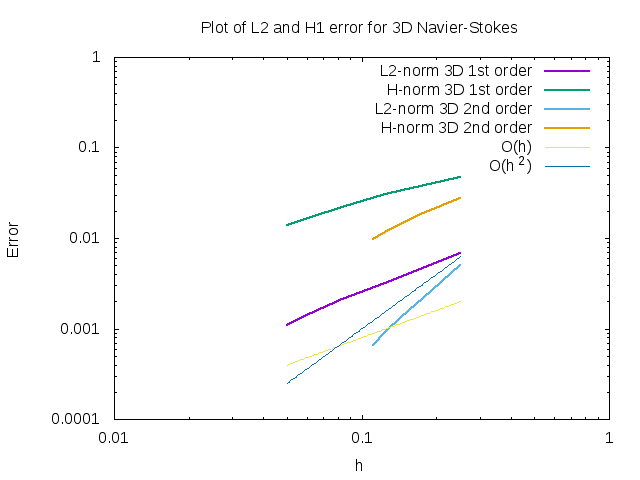
\includegraphics[width=1\linewidth]{NS_3D/error_NS_3D}
	\caption{Compare $ L^{2} $ and $ H^{1} $ norm in cubic domain}
	\label{fig:errorns3d}
\end{figure}

From the plot, we can see that Adam-Bashforth method gives second order error. Other words, this method will provide better solution with smaller error increment. 

\subsubsection{Cylindrical domain}
Choosing $ a=1/8 $, $ \epsilon_{i}=1 $, $ \beta_{i}=1 $ for $ (i=1, \dots,6) $.
\[ \Omega = \{ x=(x,y,z) \in \R^3 ; -a\leq z \leq 4a, \sqrt{x^2+y^2} < 1 \} \]
and $ u=0 $ on the boundary, cylindrical domain with with ratio 1, 0.4, and 0.1 is build. We look for $ L^{2} $ and $ H^{1} $ norm for second order in time such that $ L^{2} = O(h) $ and $ H^{1} = O(h) $ is expected for $ dt = \dfrac{\sqrt{h}}{16}. $

\begin{figure}[h!]
	\centering
	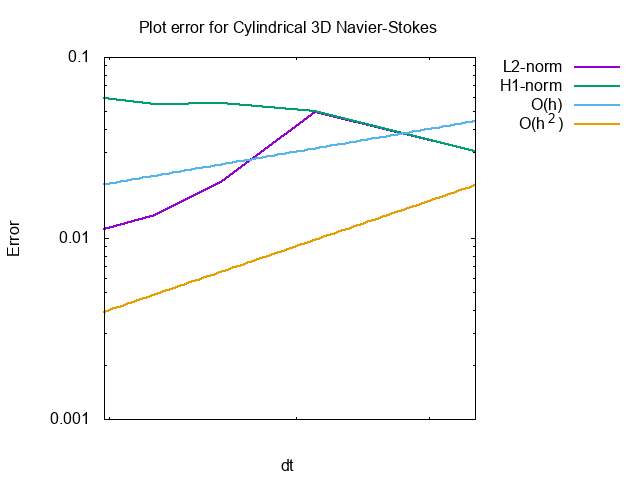
\includegraphics[width=1\linewidth]{NS_3D/error_cyl}
	\caption{Compare $ L^{2} $ and $ H^{1} $ norm}
	\label{fig:errorcyl}
\end{figure}

From the Figure (\ref{fig:errorcyl}), the $ L^{2} $ norm is seems correct before bigger $ dt $. But, $ H^{1} $ norm is still not correct. I expect, the definition space for the exact in the program is playing part for the decreasing order.

\subsection{Cylindrical and curved cylindrical domain with initial}
Choose $ a=1/8 $, $ \epsilon_{i}=1 $, $ \beta_{i}=1 $ for $ (i=1, \dots,6) $.
\[ \Omega = \{ x=(x,y,z) \in \R^3 ; -a\leq z \leq 4a, \sqrt{x^2+y^2} < 1 \} \]
and $ u=0 $ on the boundary. We have the initial
\begin{eqnarray}\nonumber
\psi(a,\epsilon,\sigma) &=& (a^{2}+\epsilon)^{\sigma}\\ \nonumber
u_{z} &=& \psi(r,\epsilon_{1},-\beta_{1})\psi(z,\epsilon_{2},-\beta_{2})\\ \nonumber
\rho &=& \psi(r,\epsilon_{3},-\beta_{3})\psi(z,\epsilon_{4},\beta_{4})\\ \nonumber
u_{0} &=& \psi(r,\epsilon_{5},-\beta_{5})\psi(z,\epsilon_{6},-\beta_{6}) \text{\hspace{1cm} (with swirl)}\\ \nonumber
u_{0} &=& 0 \text{ \hspace{5cm}(no swirl) }\\ \nonumber
u_{r} &=& sign(z)\rho u_{z}
\end{eqnarray}
\subsubsection{Cylindrical domain}
The error shown in the Figure (\ref{fig:errortornado}) is \textbf{still not correc}t. I expect it happened because the artificial solution is not fit with the condition for given initial condition.
\begin{figure}[h!]
	\centering
	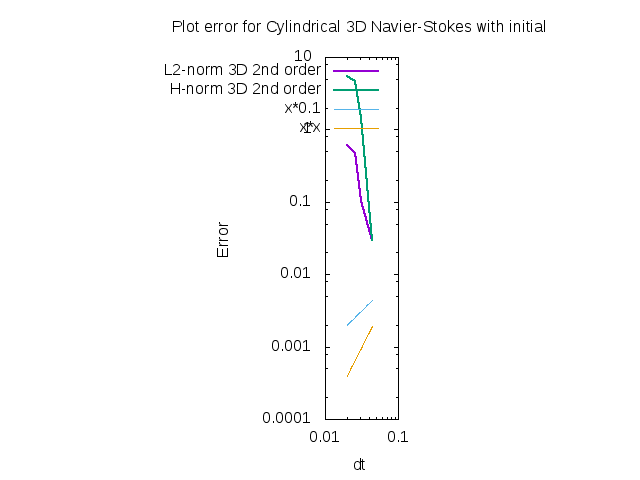
\includegraphics[width=1\linewidth]{NS_3D/error_tornado}
	\caption{Compare $ L^{2} $ and $ H^{1} $ norm}
	\label{fig:errortornado}
\end{figure}
\begin{figure}[h!]
	\centering
	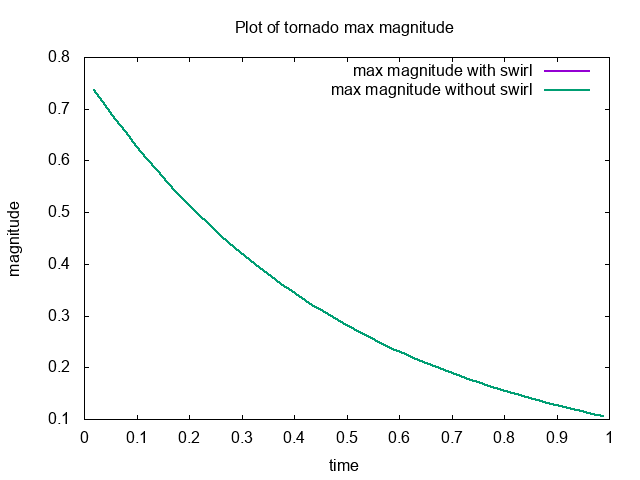
\includegraphics[width=1\linewidth]{NS_3D/magnitude_tornado}
	\caption{Maximum of $ u $ }
	\label{fig:magnitudetornado}
\end{figure}

\subsubsection{Curved cylindrical domain}
The curved domain is buid by the 
As the simulation in cylindrical domain, the error shown in the Figure (\ref{fig:errorcurved}) is \textbf{still not correct}. I expect it happened because the artificial solution is not fit with the condition for given initial condition.
\begin{figure}[h!]
	\centering
	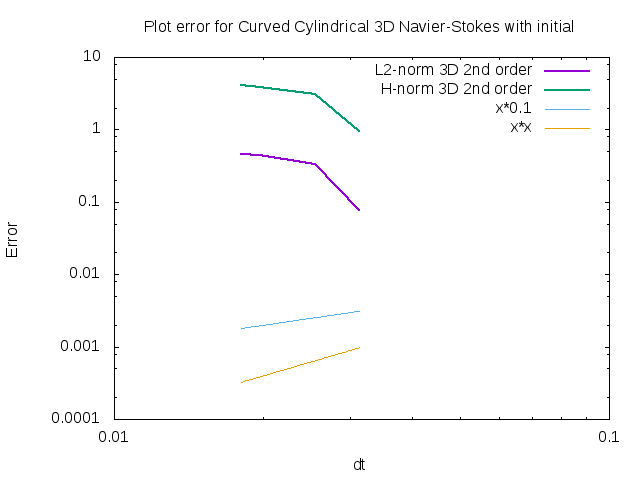
\includegraphics[width=1\linewidth]{NS_3D/error_curved}
	\caption{Compare $ L^{2} $ and $ H^{1} $ norm}
	\label{fig:errorcurved}
\end{figure}
\begin{figure}[h!]
	\centering
	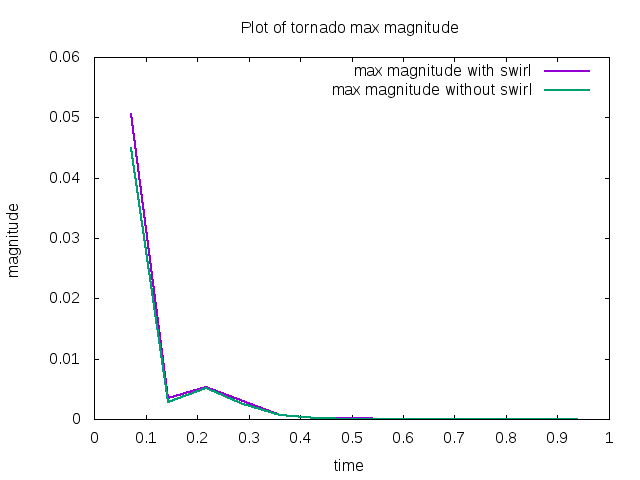
\includegraphics[width=1\linewidth]{NS_3D/curved}
	\caption{Maximum of $ u $}
	\label{fig:curved}
\end{figure}

Even through the simulation of artificial exact solution is done. There are still some doubts on the solution or the boundary conditioning. But in the movie, we could see the swirl is happening

\newpage
\section{Simulation of Tornadoes}

\subsection{Cylindrical domain}
\subsubsection{With swirl}
\begin{figure}[h!]
	\centering
	\includegraphics[width=0.8\linewidth]{../../july/Tornado_withswirl}
	\caption{}
	\label{fig:tornadowithswirl}
\end{figure}
\subsubsection{Without swirl}
\begin{figure}[h!]
	\centering
	\includegraphics[width=0.8\linewidth]{../../july/Tornado_noswirl}
	\caption{}
	\label{fig:tornadonoswirl}
\end{figure}


\subsection{Curved cylindrical domain}
\subsubsection{With swirl}
\begin{figure}[h!]
	\centering
	\includegraphics[width=0.8\linewidth]{../../july/Curved_withswirl}
	\caption{}
	\label{fig:curvedwithswirl}
\end{figure}

\subsubsection{Without swirl}
\begin{figure}[h!]
	\centering
	\includegraphics[width=0.8\linewidth]{../../july/Curved_noswirl}
	\caption{}
	\label{fig:curvednoswirl}
\end{figure}


\end{document}
